\subsection{Command-Service}
\label{subsec:implementation:commandService}
 Ähnlich wie beim \textit{Query-Service}, wird auch beim \textit{Command-Service} für jeden ankommenden Befehl ein eigener Actor gestartet, der für einen speziellen Typ von Anfrage zuständig ist. Es gibt auch hier für jeden möglichen Befehl einen eigenen Actor, welcher die Logik des Kommandos beinhaltet. Jedoch werden in der Implementierung der einzelnen Kommandos meist neue Befehle an einen oder mehrere zuständige Actors aus dem Domain-Service erzeugt und weitergeleitet. \\
% * <feitzinger.magdalena@gmail.com> 2018-05-18T06:03:36.815Z:
% 
% > Jedoch werden in der Implementierung der einzelnen Kommandos meist neue Befehle an einen oder mehrere zuständige Actors aus dem Domain-Service erzeugt und weitergeleitet
% Präzisieren! 
% 
% ^.
% * <feitzinger.magdalena@gmail.com> 2018-05-18T06:02:47.640Z:
% 
% > Ähnlich wie beim \textit{Query-Service}, wird auch beim \textit{Command-Service} für jeden ankommenden Befehl ein eigener Actor gestartet, der für einen speziellen Typ von Anfrage zuständig ist. Es gibt auch hier für jeden möglichen Befehl einen eigenen Actor welcher die Logik des Kommandos beinhaltet.
% Beide Sätze haben dieselbe Aussage. 
% 
% ^.
 In der vorliegenden Implementierung gibt es folgende unterschiedliche Typen von Kommandos, welche alle durch einen \textit{CommandHandler} repräsentiert werden:
 \begin{enumerate}
     \item Flüge erstellen
     \item Flug vorbereiten
     \item Ticket reservieren
     \item Ticket buchen
 \end{enumerate}
Die Abbildung \ref{fig:implementation:commandActorModel} zeigt den Aufbau des \textit{Command-Service}. Die  Geschäftslogik ist  in den Actoren des \textit{Domain Serice} beherbergt. Somit ist die Tätigkeit der einzelnen \textit{CommandHandler} darauf begrenzt, die betroffenen Actoren im \textit{Domain Serice} über die gewünschte Tätigkeit zu informieren und diese  auszuführen. 
 \begin{figure}
    \centering
    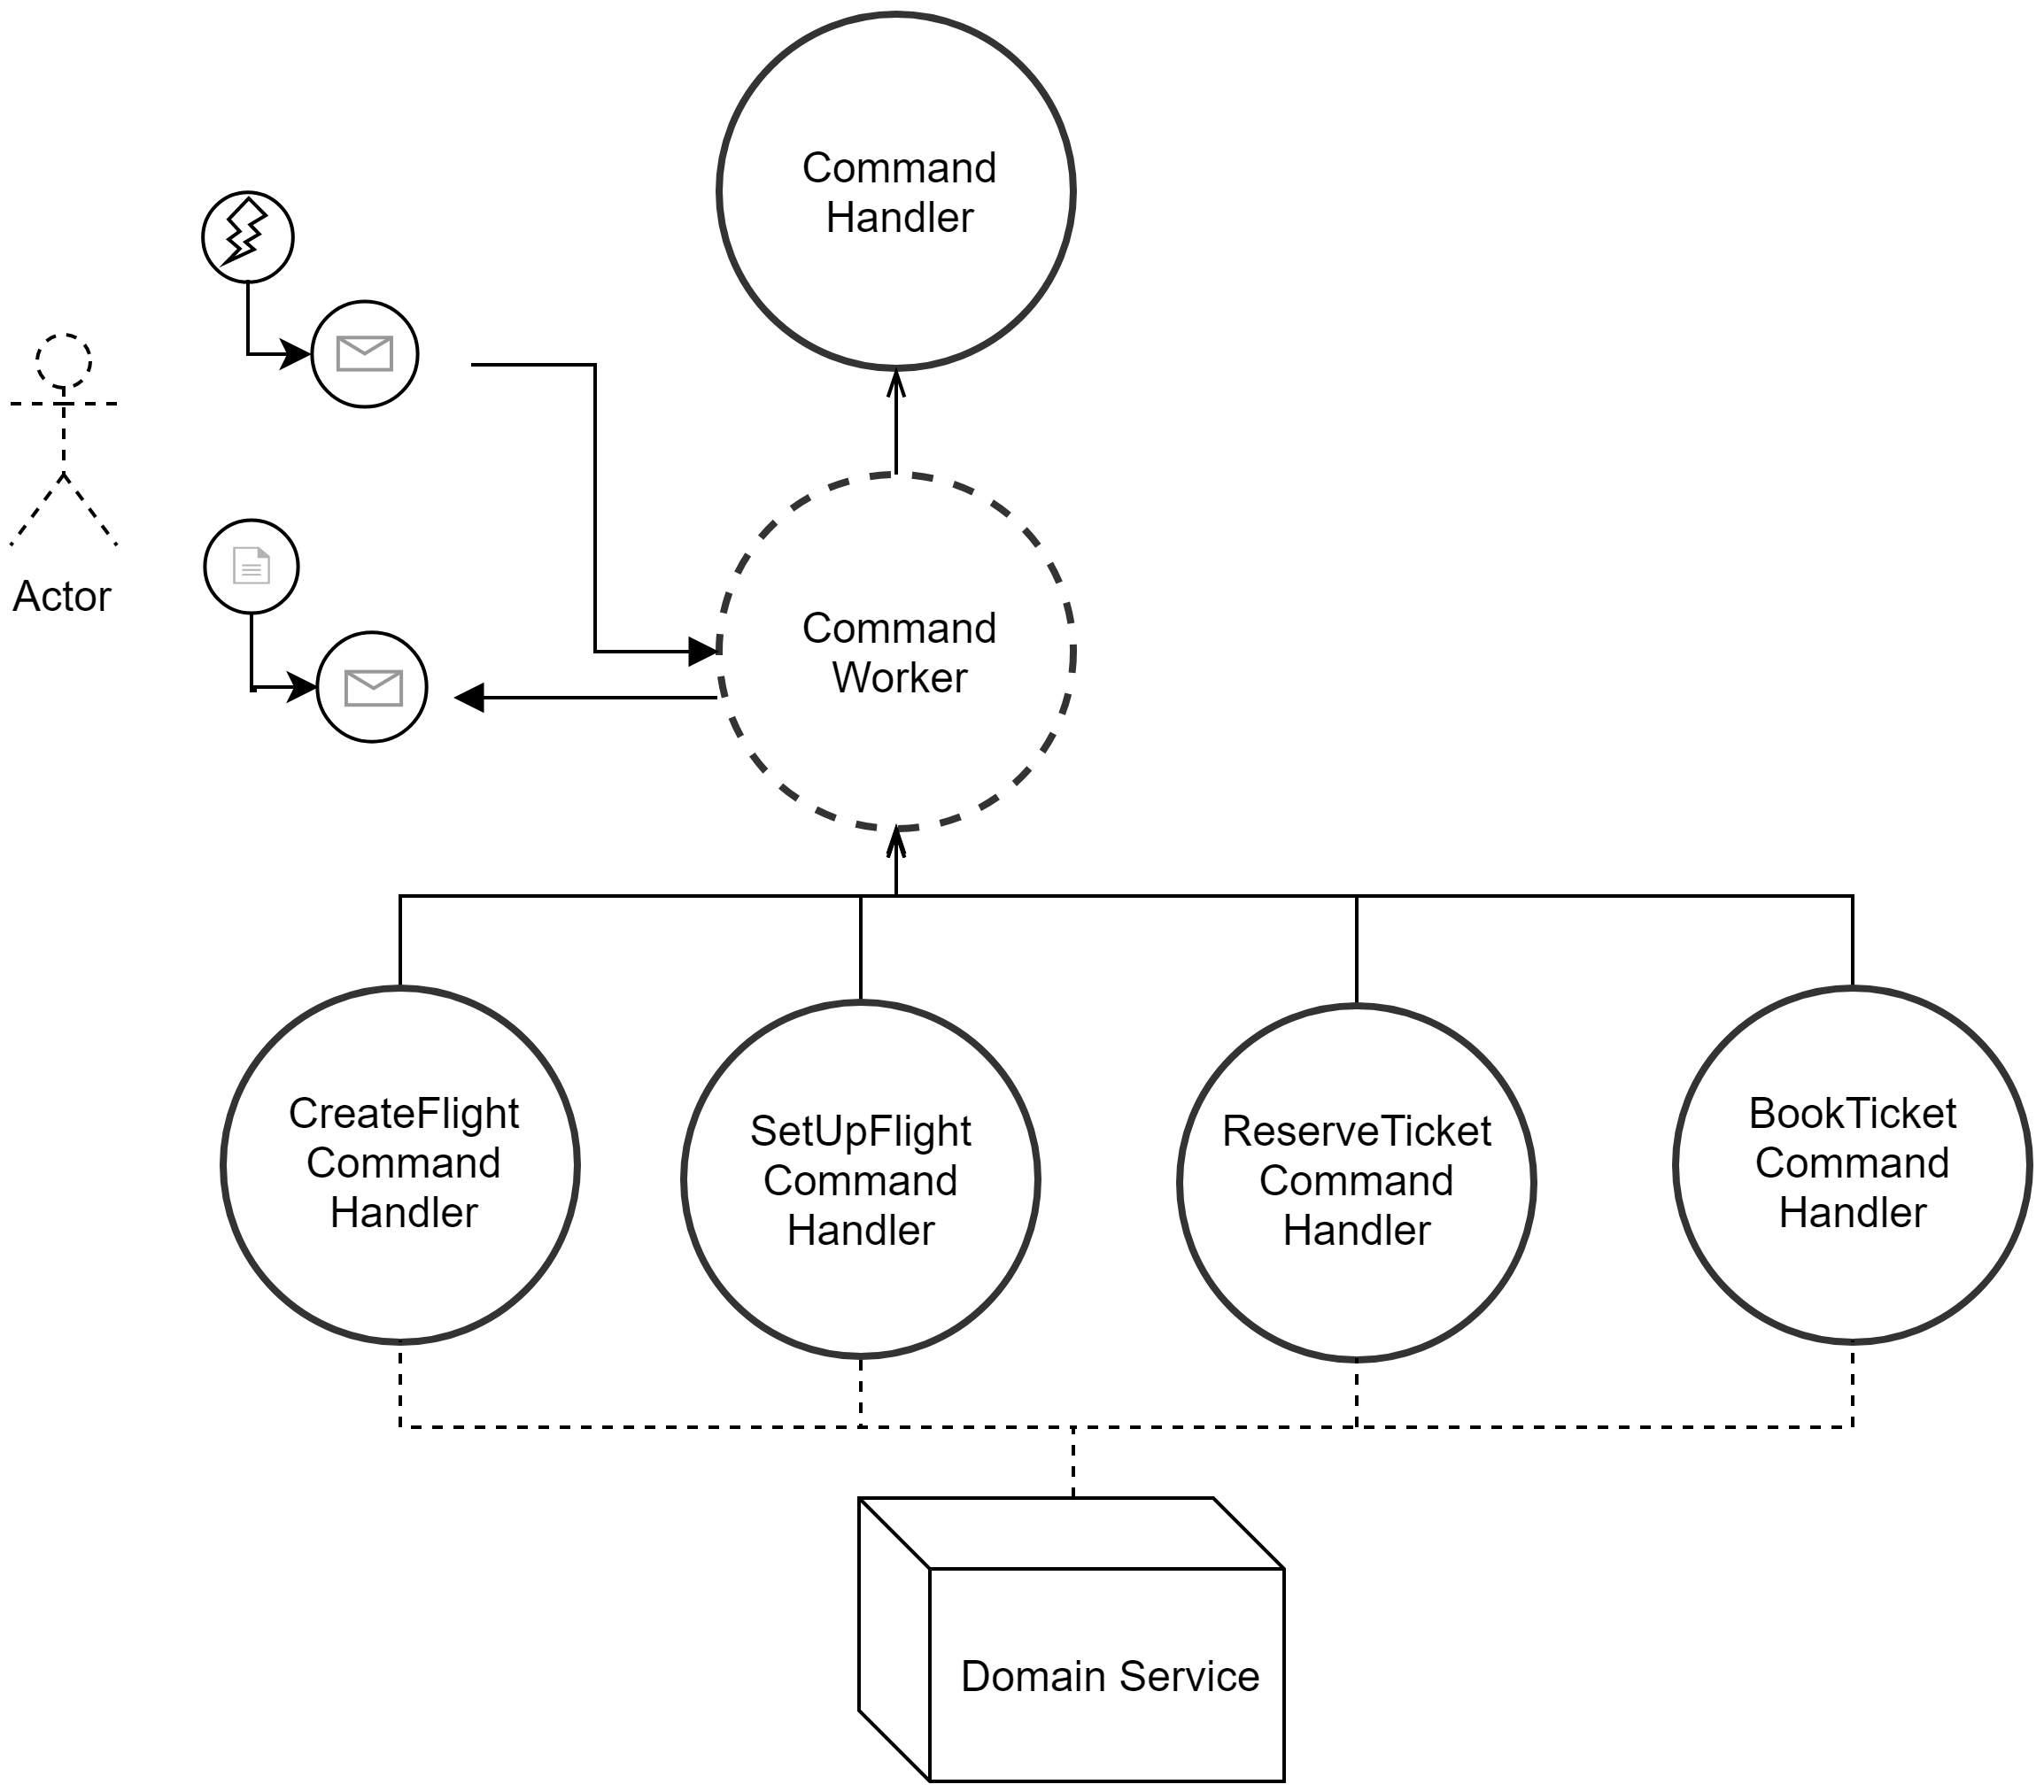
\includegraphics[width=0.8\linewidth]{gfx/implementation/CommandServiceActorModel}
    \caption{Der Aufbau des \textit{Command-Service} beinhaltet die Logik der einzelnen Befehle und leitete weitere Befehle an den \textit{Domain-Service} weiter }
    \label{fig:implementation:commandActorModel}
\end{figure} 

